%!TEX root = ../main.tex
\chapter{Matplotlib} \label{chap:matplotlib}

Matplotlib ist eine Bibliothek für Python mit deren Hilfe  Kennlinien und Diagramme mit nur wenigen Zeilen Code erzeugt werden können.  Nach dem Importieren der Bibliothek, muss der Funktion plot nur y-Werte übergeben werden. Die x-Werte werden inkrementell in einer schritten hinzugefügt. Unterscheiden sich die eigenen x-Werte jedoch von den automatisch erzeugten, können auch diese der Funktion übergeben werden. Das in Abb. \ref{img:MPL1} dargestellte Diagramm würde somit identisch aussehen wenn ich der Funktion nur die y-Werte übergeben würde. 

\begin{figure}[!htb]
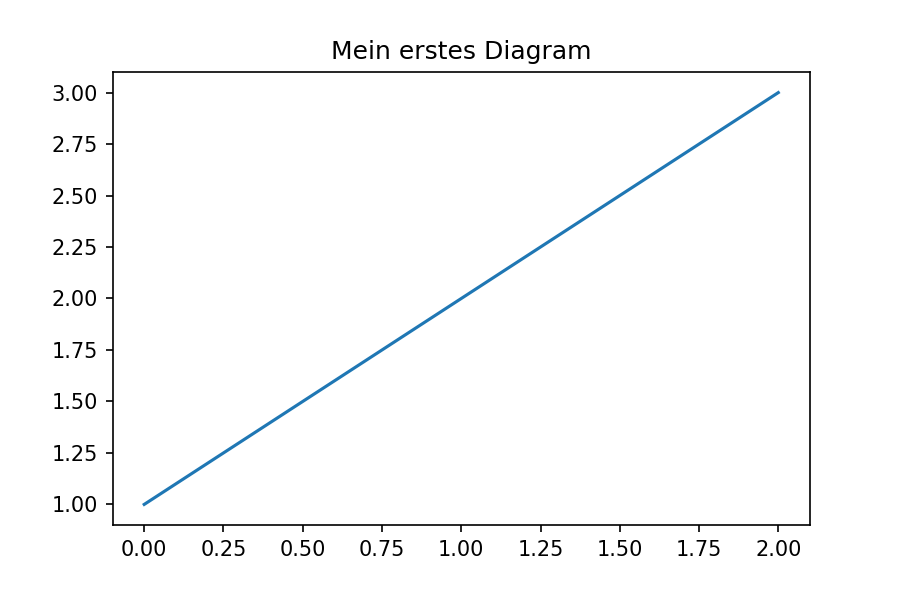
\includegraphics{MeinErstesDiagramm.png}
\caption{Mein erstes Diagramm in Jupyter Notebook mit matplotlib }
\label{img:MPL1}
\end{figure}

Die Achsen lassen sich beschriften \texttt{xlabel,ylabel} man kann die Textgröße fontsize  bestimmen, sowie die Position \texttt{verticalalignment, horizontalalignment} und den Abstand zur Achsenlinie \texttt{labelpad}. Die Achseneinteilung lässt sich umbenennen dezimieren und rotieren. Matplotlib ist kompatibel mit Latex. 

\begin{figure}[!htb]
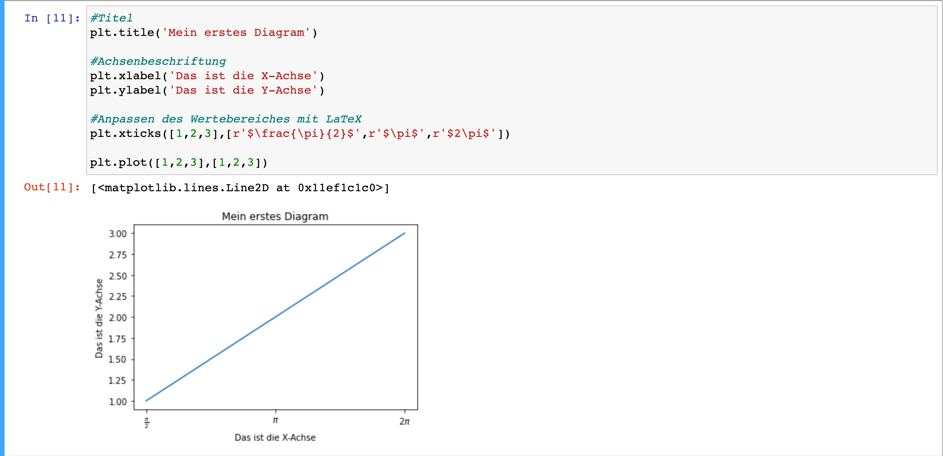
\includegraphics{Diagramm_mit_Beschriftung.png}
\caption{Diagramm mit Beschriftung}
\label{img:DiagrammMitBeschriftung}
\end{figure}

Um eine Funktion mit matplotlib darzustellen muss  eine Wertetabelle erstellt werden. Mithilfe einer Funktion wird der Definitionsbereich festgelegt.

\begin{figure}[!htb]
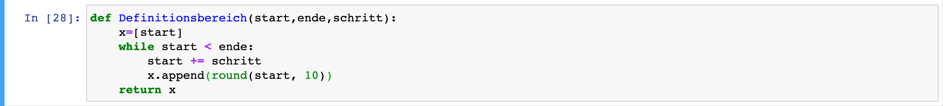
\includegraphics{Definitionsbereich.png}
\caption{Funktion: Definitionsbereich}
\label{img:Definitionsbereich}
\end{figure}

Um die Wertetabelle zu vervollständigen, wird durch eine Funktion der Wertebereich bestimmt. Betrachten wir als Beispiel eine Parabel. Der Funktion \texttt{Parabel(x)} werden die x-Werte übergeben im Bereich von -3 bis 3, die x-Werte werden mithilfe der Funktion \texttt{Definitionsbereich(-3,3,0.1)} erstellt. Als Rückgabewert liefert die Funktion \texttt{Parabel(x)} die y-Werte. Übergeben wir der Funktion \texttt{plt.plot(x,y)} die x- und y-Werte. Sie als Ausgabe den Funktionsgraph zurück.

\begin{figure}[!htb]
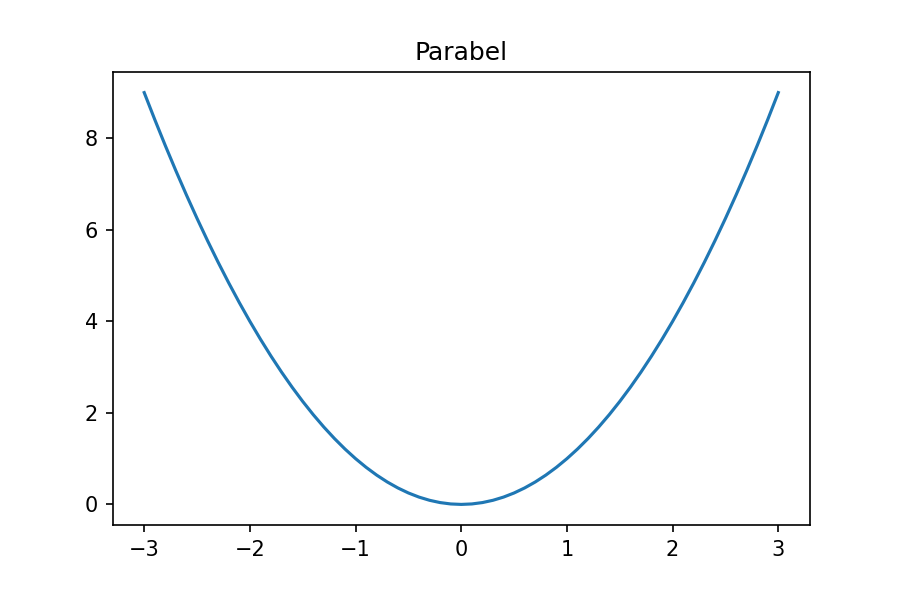
\includegraphics[scale=1]{Parabel.png}
\caption{Parabel}
\label{img:Parabel}
\end{figure}

\section{Objekte von Matplotlib} \label{sec:Objekte von Matplotlib}

Eine matplotlib Grafik beinhaltet eine in sich geschachtelte Objekthierarchie. Das Figure Objekt ist das äußerste Fenster einer matplotlib Grafik. In einem Figure Objekt können mehrere Axes Objekte erzeugt werden, die ein Diagramm darstellen.

\begin{figure}[!htb]
\centering
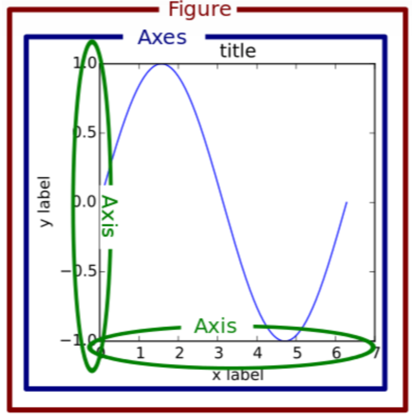
\includegraphics[scale=1]{FigureAufbau.png}
\caption{Aufbau von einem matplotlib Objekt \cite{matplotlib}}
\label{img:FigureObjekt}
\end{figure}

Anstelle von \texttt{plt.plot()} erstellen wir eine Objekt Figure dem wir ein Axes Objekt als unter Plot hinzufügen.

\begin{figure}[!htb]
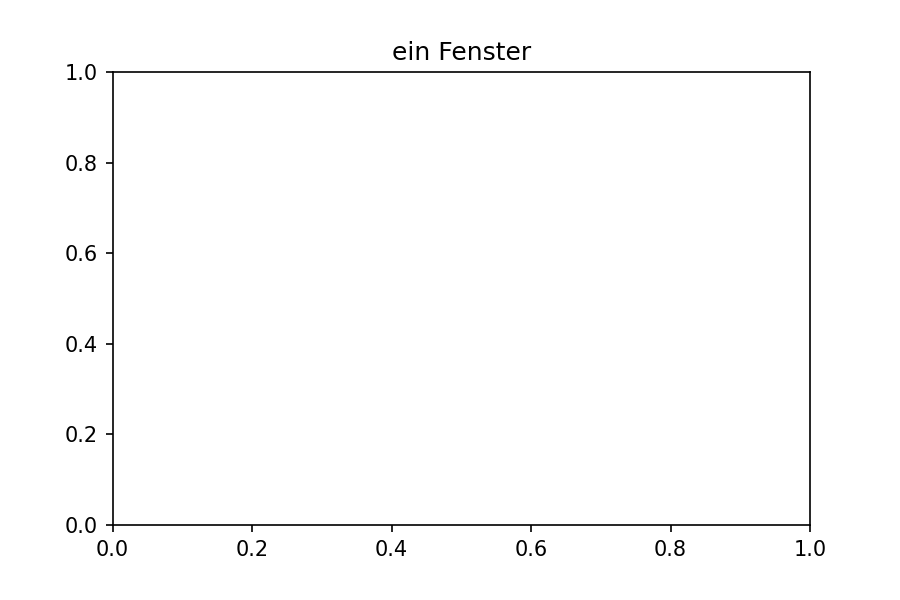
\includegraphics[scale=1]{EinFigureEinAxes.png}
\caption{Ein Figure Objekt mit einem Axes Objekt}
\label{img:EinFigureEinAxes}
\end{figure}

Eine Figure Objekt kann mehrere Axes Objekte enthalten. Ein Figure Objekt kann in Spalten und Zeilen unterteilt werden in jedem Feld kann sich ein Axes Objekt befinden. Die einzelnen Axes Objekte werden der Reihe nach von links nach rechts nummeriert und so angesprochen add\_subplot(Reihenanzahl, Spaltenanzahl, Nummer) .  In Abbildung \ref{img:EinFigureEinAxes} wurde das Figure Objekt in eine Spalte und eine Reihe unterteilt somit ergibt sich nur ein Feld mit einem Axes Objekt. Wenn wir zwei Axes Objekte neben einander anlegen wollen müssen wir die Methode add\_subplot() zweimal aufrufen mit einer Zeile und zwei Spalten. 
Exemplarisch wurde hier dargestellt das die Form und Farbe der Linie beeinflusst werden kann. 

\begin{figure}[!htb]
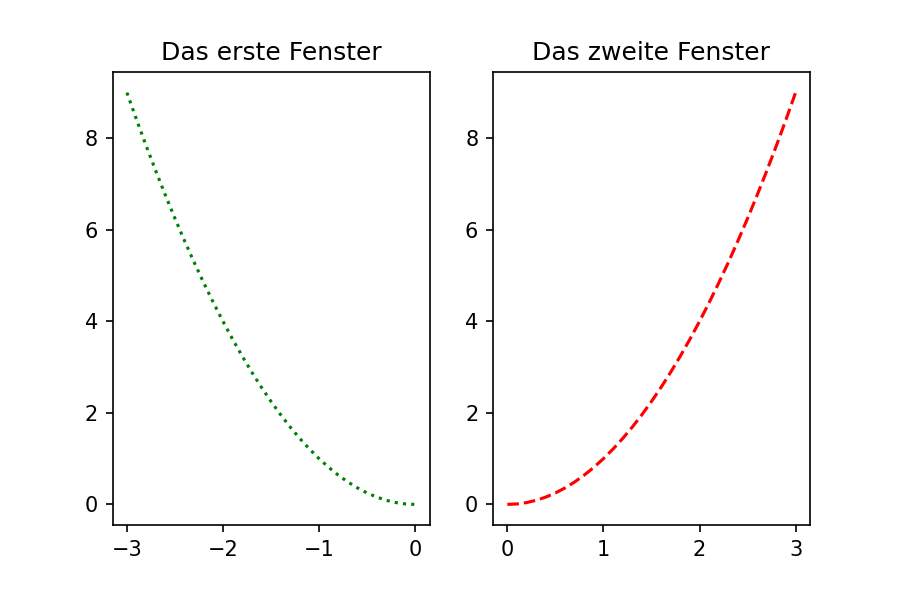
\includegraphics[scale=1]{ZweiAxesEinFigure.png}
\caption{Zwei Axes Objekte in einem Figure Objekt}
\label{img:ZweiAxesEinFigure}
\end{figure}

Möchte man zwei Linien darstellen muss man dafür nicht zwangsläufig zwei Axes Objekte erzeugen. Es können beliebig viele Linien in einem Axes Objekt erzeugt werden, zur übersichtlichen Darstellung empfiehlt sich eine Legende die mit \texttt{labe}l und \texttt{.legend()} dargestellt werden kann

\begin{figure}[!htb]
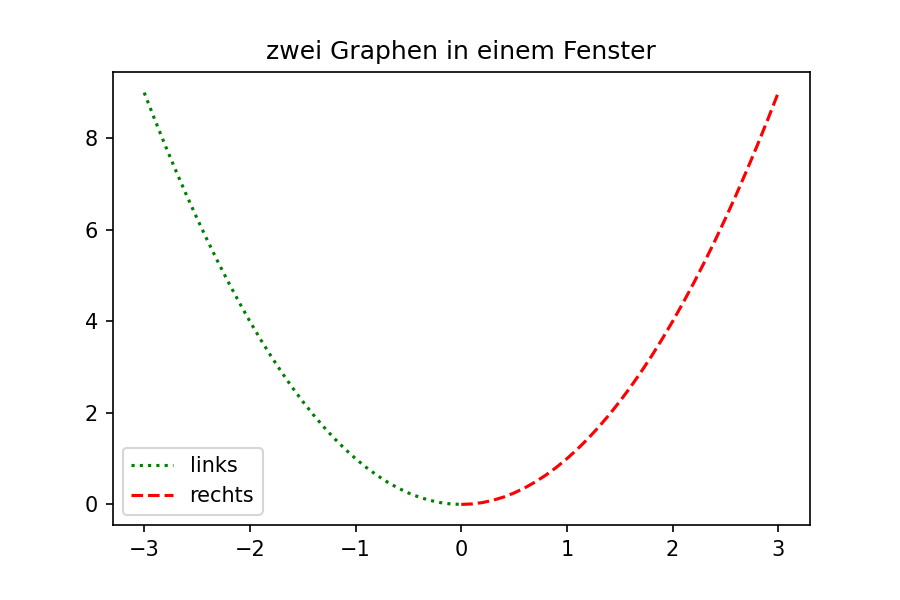
\includegraphics[scale=1]{ZweiGraphenEinAxes.png}
\caption{Zwei Graphen in einem Axes Objekt}
\label{img:ZweiGraphenEinAxes}
\end{figure}

Damit jedes Axes Objekt nicht einzeln erstellt werden muss, kann man alternativ die Methode \texttt{subplots()} verwenden.
Übergibt man der Methode Zeilen und Spalten Anzahl liefert sie als Rückgabewert ein Figure Objekt und die Axes Objekte, die in einem Array gespeichert werden können

\begin{figure}[!htb]
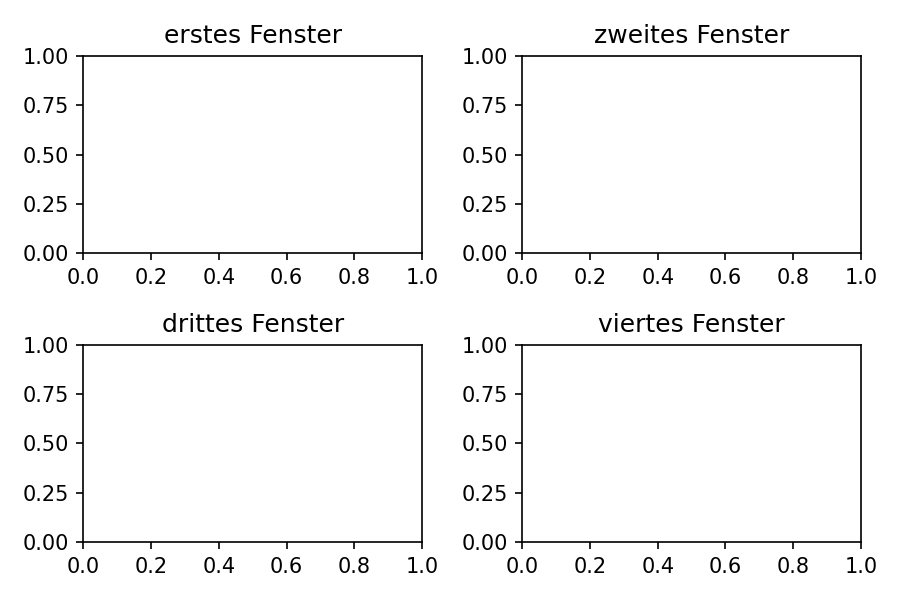
\includegraphics[scale=1]{AxesArray.png}
\caption{Axes Objekt Array}
\label{img:AxesArray}
\end{figure}


\section{I-U Kennlinie} \label{sec: IUKennlinie}

In dieser Ausarbeitung werden I-U-Kennlinien vermehrt vorkommen. Für eine I-U-Kennlinie wird die Y-Achse mit  $I_{D}\, in\, A $  beschriftet. Die Beschriftung soll Horizontal ausgerichtet und am oberen Ende der Achse  positioniert werden . Die X-Achse wird mit $U_{D}\,  in\, V$ beschriftet und am rechten Ende der Achse positioniert. Des weiteren muss die obere und rechte  Begrenzungslinie entfernt werden. Zum Schluss benötigt der Graph noch eine Überschrift. Da diese Kriterien für alle I-U-Kennlinien gelten wird eine Funktion geschrieben. 

\begin{figure}[!htb]
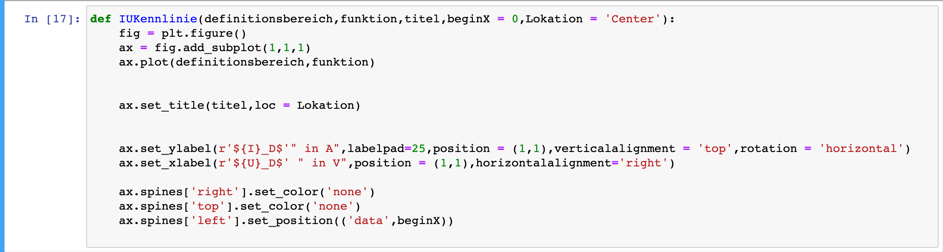
\includegraphics[scale=1]{IUKennlinie.png}
\caption{Funktion zum Erzeugen einer I-U Kennlinie}
\label{img:IUKennlinie}
\end{figure}


